\documentclass[tikz,border=3mm]{standalone}
\usetikzlibrary{positioning, shapes.geometric, arrows.meta, calc, fit, backgrounds}

\begin{document}
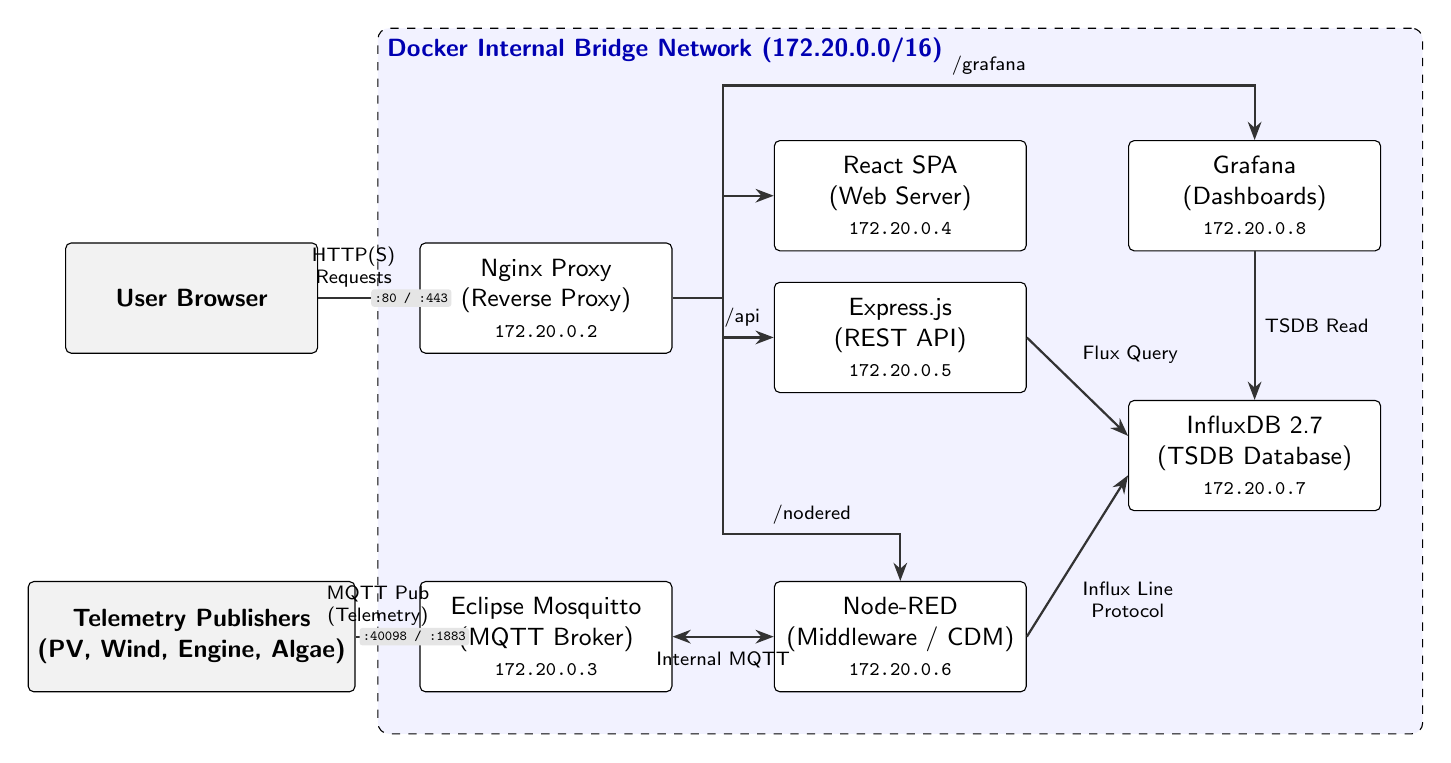
\begin{tikzpicture}[
    box/.style={draw, fill=white, minimum width=3.2cm, minimum height=1.4cm, align=center, font=\sffamily\small, rounded corners=2pt},
    extbox/.style={draw, fill=black!5, minimum width=3.2cm, minimum height=1.4cm, align=center, font=\sffamily\small\bfseries, rounded corners=2pt},
    arrow/.style={-Stealth, thick, draw=black!80},
    doublearrow/.style={Stealth-Stealth, thick, draw=black!80},
    lbl/.style={font=\sffamily\scriptsize, align=center},
    port/.style={font=\ttfamily\tiny, fill=gray!20, inner sep=1.2pt, rounded corners=1pt}
]

    % ================= LEFT COLUMN: EXTERNAL CLIENTS =================
    \node[extbox] (Browser) at (0, 2.5) {User Browser};
    \node[extbox] (Assets) at (0, -1.8) {Telemetry Publishers\\(PV, Wind, Engine, Algae)};

    % ================= DOCKER INTERNAL NETWORK (CONTAINERS) =================
    
    % Nginx Gateway Container
    \node[box] (Nginx) at (4.5, 2.5) {Nginx Proxy\\(Reverse Proxy)\\\scriptsize\texttt{172.20.0.2}};
    
    % Mosquitto Broker Container
    \node[box] (Mosquitto) at (4.5, -1.8) {Eclipse Mosquitto\\(MQTT Broker)\\\scriptsize\texttt{172.20.0.3}};

    % Web Server and Backend API Containers
    \node[box] (ReactSPA) at (9.0, 3.8) {React SPA\\(Web Server)\\\scriptsize\texttt{172.20.0.4}};
    \node[box] (Express) at (9.0, 2.0) {Express.js\\(REST API)\\\scriptsize\texttt{172.20.0.5}};
    
    % Middleware Orchestrator Container
    \node[box] (NodeRED) at (9.0, -1.8) {Node-RED\\(Middleware / CDM)\\\scriptsize\texttt{172.20.0.6}};

    % Databases and Visualizers
    \node[box] (Grafana) at (13.5, 3.8) {Grafana\\(Dashboards)\\\scriptsize\texttt{172.20.0.8}};
    \node[box] (InfluxDB) at (13.5, 0.5) {InfluxDB 2.7\\(TSDB Database)\\\scriptsize\texttt{172.20.0.7}};

    % Dummy coordinate to expand Docker boundary box upwards to include the Nginx -> Grafana routing line
    \coordinate (DockerTop) at (9.0, 5.4);

    % ================= NETWORKS AND BOUNDARIES =================
    
    % Docker bridge network background group
    \begin{scope}[on background layer]
        \node[draw, dashed, fill=blue!5, rounded corners=4pt, inner sep=15pt,
              fit=(Nginx) (Mosquitto) (ReactSPA) (Express) (NodeRED) (Grafana) (InfluxDB) (DockerTop)] (DockerNet) {};
    \end{scope}
    
    \node[font=\sffamily\small\itshape\bfseries, text=blue!70!black, anchor=north west] at (DockerNet.north west) {Docker Internal Bridge Network (172.20.0.0/16)};

    % ================= DRAW CONNECTIONS =================

    % External requests
    \draw[arrow] (Browser.east) -- (Nginx.west) 
        node[pos=0.35, above, lbl] {HTTP(S)\\Requests} 
        node[pos=0.92, port] {:80 / :443};
        
    \draw[arrow] (Assets.east) -- (Mosquitto.west) 
        node[pos=0.35, above, lbl] {MQTT Pub\\(Telemetry)} 
        node[pos=0.92, port] {:40098 / :1883};

    % Nginx Gateway Routing Bus Split
    \coordinate (BusSplit) at (6.75, 2.5);
    \draw[thick, draw=black!80] (Nginx.east) -- (BusSplit);
    
    % Routing lines from Bus Split
    \draw[arrow] (BusSplit) |- (ReactSPA.west);
    
    \draw[arrow] (BusSplit) |- (Express.west);
    \node[above, lbl] at ($(Express.west)-(0.4,0)$) {/api};
    
    % Rerouted Node-RED path to connect to top border, avoiding Mosquitto <-> Node-RED connection
    \draw[arrow] (BusSplit) |- (9.0, -0.5) -- (NodeRED.north);
    \node[above, lbl] at (7.875, -0.5) {/nodered};
    
    \draw[arrow] (BusSplit) |- (13.5, 5.2) -- (Grafana.north);
    \node[above, lbl] at (10.125, 5.2) {/grafana};

    % Ingestion pipeline data flow (double arrow between Mosquitto and Node-RED)
    \draw[doublearrow] (NodeRED.west) -- (Mosquitto.east) 
        node[midway, below, lbl, yshift=-2pt] {Internal MQTT};
        
    \draw[arrow] (NodeRED.east) -- ($(InfluxDB.west)-(0,0.25)$) 
        node[pos=0.45, below right, lbl, yshift=-0.1cm] {Influx Line\\Protocol};

    % Query & Visualization connections
    \draw[arrow] (Express.east) -- ($(InfluxDB.west)+(0,0.25)$) 
        node[pos=0.45, above right, lbl, yshift=0.1cm] {Flux Query};
        
    \draw[arrow] (Grafana.south) -- (InfluxDB.north) 
        node[midway, right, lbl] {TSDB Read};

\end{tikzpicture}
\end{document}
